\chapter{Trabalhos Relacionados}
\label{cap:trabalhos-relacionados}

Integer non lacinia magna. Aenean tempor lorem tellus, non sodales nisl commodo ut. Proin mattis placerat risus sit amet laoreet. Praesent sapien arcu, maximus ac fringilla efficitur, vulputate faucibus sem. Donec aliquet velit eros, sit amet elementum dolor pharetra eget. Integer eget mattis libero

\section{Trabalho Relacionado A}
\label{sec:trabalho-relacionado-a}

\lipsum[10]

	\begin{figure}[h!]
		\centering
		\Caption{\label{fig:exemplo-1} Lorem ipsum dolor sit amet, consectetur adipiscing elit. Suspendisse commodo lectus et augue elementum varius.}	
		\UNIFORfig{}{
			\fbox{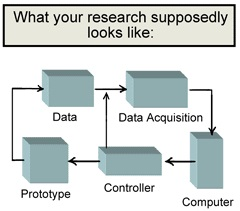
\includegraphics[width=8cm]{figuras/figura-1}}
		}{
			\Fonte{Elaborado pelo autor}
		}	
	\end{figure}
	
\lipsum[11]

\section{Trabalho Relacionado B}
\label{sec:trabalho-relacionado-b}

Integer non lacinia magna. Aenean tempor lorem tellus, non sodales nisl commodo ut. Proin mattis placerat risus sit amet laoreet. Praesent sapien arcu, maximus ac fringilla efficitur, vulputate faucibus sem. Donec aliquet velit eros, sit amet elementum dolor pharetra eget. Integer eget mattis libero. Praesent ex velit, pulvinar at massa vel, fermentum dictum mauris. Ut feugiat accumsan augue, et ultrices ipsum euismod vitae

	\begin{figure}[h!]
		\centering
		\Caption{\label{fig:exemplo-2} Maecenas luctus augue odio, sed tincidunt nunc posuere nec}	
		\UNIFORfig{}{
			\fbox{
\includegraphics[width=8cm]{figuras/figura-2}}
		}{
			\Fonte{Elaborado pelo autor}			
		}	
	\end{figure}

Nunc ac pretium dui. Mauris aliquam dapibus nulla ac mattis. Aenean non tortor volutpat, varius lectus vitae, accumsan nibh. Cras pretium vestibulum enim, id ullamcorper tortor ultrices non. Integer sodales viverra faucibus. Curabitur at dui lacinia, rhoncus lacus at, blandit metus. Integer scelerisque non enim quis ornare.

	\begin{quadro}[h!]	
		\centering
		\Caption{\label{qua:exemplo-1} Praesent ex velit, pulvinar at massa vel, fermentum dictum mauris. Ut feugiat accumsan augue}		
		\UNIFORqua{}{
			\begin{tabular}{|c|c|l|l|}
				\hline
				Quisque & pharetra & tempus & vulputate \\
				\hline
				E1 & Complete coverage by a single transcript & Both  & Complete\\
				\hline
				E2 & Complete coverage by more than & Both splice sites & Complete\\
				\hline
				E3 & Partial coverage & Both splice sites & Both \\				
				\hline
			\end{tabular}
		}{
			\Fonte{Elaborado pelo autor}
		}
	\end{quadro}
	
\lipsum[20]

	
	\begin{quadro}[h!]	
		\centering
		\Caption{\label{qua:exemplo-2} Duis faucibus, enim quis tincidunt pellentesque}		
		\UNIFORqua{}{
			\begin{tabular}{|c|c|}
				\hline
				Quisque & pharetra \\
				\hline
				E1 & Complete coverage by a single transcript \\
				\hline
				E2 & Complete coverage by more than \\
				\hline
				E3 & Partial coverage \\
				\hline
				E4 & Partial coverage \\
				\hline
				E5 & Partial coverage \\
				\hline
				E6 & Partial coverage \\
				\hline
				E7 & Partial coverage \\
				\hline
			\end{tabular}
		}{
			\Fonte{Elaborado pelo autor}
		}
	\end{quadro}

\lipsum[21]

Integer non lacinia magna. Aenean tempor lorem tellus, non sodales nisl commodo ut. Proin mattis placerat risus sit amet laoreet. Praesent sapien arcu, maximus ac fringilla efficitur, vulputate faucibus sem. Donec aliquet velit eros, sit amet elementum dolor pharetra eget. Integer eget mattis libero.
\Gls{ambiguidade}
\Gls{braile}
\Gls{coerencia}
\Gls{dialetos}
\Gls{elipse}
\Gls{locucao-adjetiva}
\Gls{modificadores}
\Gls{paronimos}
\Gls{sintese}
\Gls{borboleta}